\documentclass{article}
\usepackage[utf8]{inputenc}
\usepackage{graphicx}
\usepackage[margin=1in]{geometry}

\title{PASIPHAE - Observation Planner Software}
\author{John Kypriotakis, Poorva Bhalerao, Siddharth Maharana}
\date{October 2018}

\begin{document}

\maketitle

\section{Introduction}
This document highlights the progress of the observation planning of PASIPHAE. 


\section{The Observation Planner Software}
\subsection{Description}
The Observation Planner Software (henceforth referred to as 'OPS') of the Polar-Areas Stellar Imaging in Polarization High-Accuracy Experiment (PASIPHAE) will be an almost entirely independent system that will handle the scheduling of observations over the complete duration of the survey, at both observing sites. Its fundamental role is to optimize the observing strategy in terms of time and other costly resources. The Observation Planner Software will choose the ‘best’ field to be observed by the telescope at a particular point of time and forward this decision to the Telescope Control with or without an operator’s approval. This technique surpasses most previously used surveying strategies such as the drift mode of the ALFALFA Survey (Giovanelli R. et al. 2005) and other multiple-pass strategies as it will continually strive to eliminate capturing of bad science images. 

\subsection{Objectives}
The general idea is to create a metric function with a set of static and dynamic input parameters as its individual terms. The value of this metric function will decide the priority of a field to be observed and an output analogous to a heat-map will be generated based on the priority for each field.
\\
\\
The software must have the following primary features:
\begin{enumerate}
\item Access to required databases concerning all input parameters;
\item An optimized algorithm and merit function taking into account all possible inputs and scalability of each individual parameter;
\item Ability to generate an optimal metric map taking into account the "cost" of choosing the next field (for example, time of slew to next field);
\item Implement a unified approach to cover the entire target sky area in coherent patches; 
\item Ability to "recover from stoppage in the middle of a night" (Delgado F. et al. 2014) in order to minimize down-time.
\end{enumerate}

\subsection{The Base Algorithm}

\begin{figure}[!ht]
\centering
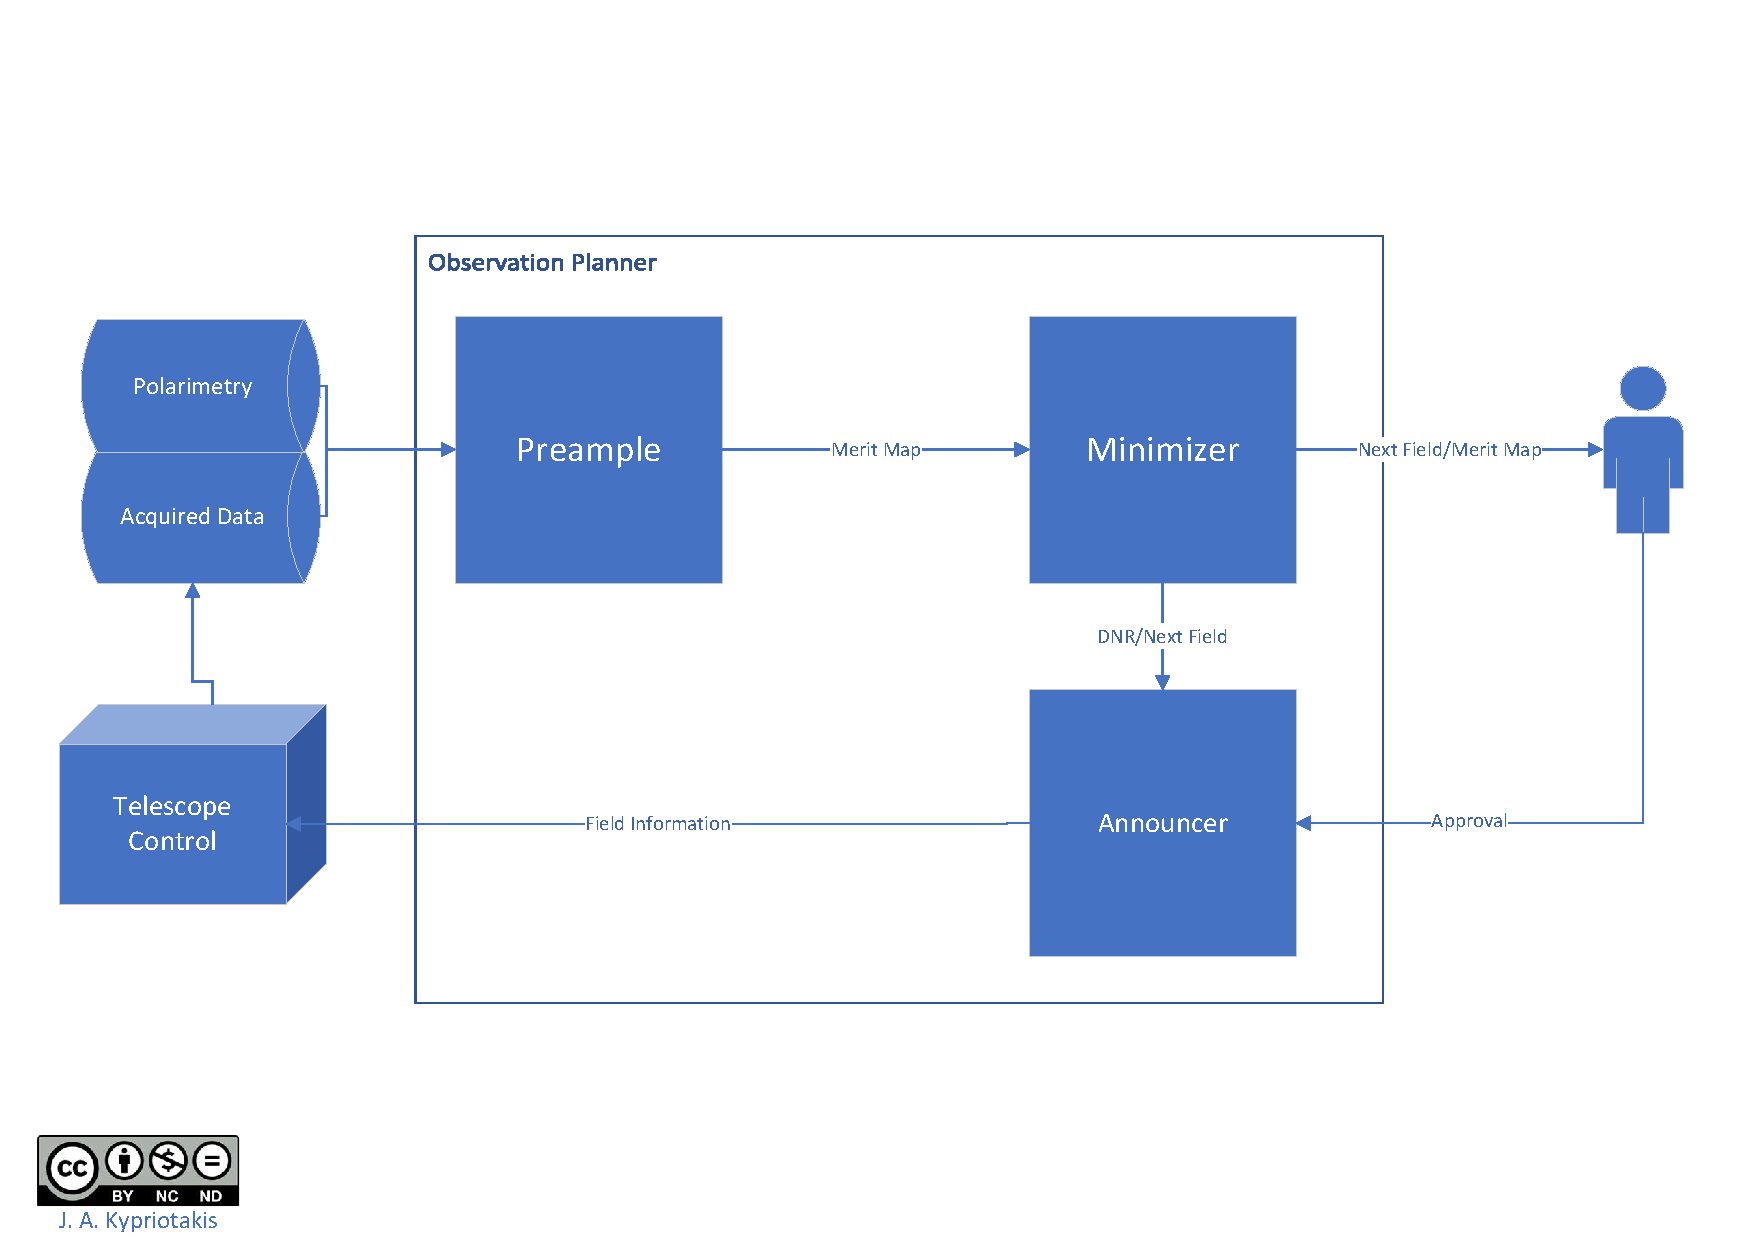
\includegraphics[width=\linewidth]{Base_new.pdf}
\caption{The base flow chart of the observation planning algorithm.}
\label{fig:baseflow}
\end{figure}

The Observation Planner will comprise of at least three main abstract  components - 1.Preample, 2.Minimizer and 3.Announcer.

\subsubsection{Preample}
The preample takes in a set of inputs (which are mentioned in a later section) from various input modules for each parameter of the metric function, computes the value of the metric function and passes a metric map to the minimizer.

\subsubsection{Minimizer}
The minimizer then looks for the field having the lowest metric i.e. the field having the highest priority (lower the metric function value, higher is its priority) and sends an approval request to the telescope operator.\newline The operator then approves this decision and the approval is passed on to the announcer.\newline In case the operator does not respond to the request within the stipulated time window, the minimizer directly outputs the next chosen field to the announcer. 

\subsubsection{Announcer}
The announcer accepts the chosen field and sends the corresponding pointing information to the Telescope Control.\\The acquired data, as one of the input modules, will in turn be fed back to the preample as an input to construct an updated metric map.

\subsection{Input Parameters to Calculate Field Priority}
The set of input modules to the Observation Planner can be divided into: Static inputs, Dynamic inputs and User Assisted inputs. A brief description of each of the inputs is provided below.

\subsubsection{Static Inputs}
\begin{enumerate}
\item Intended survey coverage\newline
    The intended survey coverage of the Northern and Southern Galactic Planes as per specification by the collaboration.
\item Location of the city\newline
    The distance of the observing sites from the nearest city is known, hence subsequent light pollution can be accounted for. 
\item Specifications and limitations of the telescope, telescope instruments and observatory dome\newline
    Specifications such as-
    \begin{enumerate}
        \item Frame size for WALOP-N (30'x30') and WALOP-S (35'x35');
        \item Speed of telescope slew;
        \item Other specifications of the telescope instrument that will affect the observing strategy.
    \end{enumerate}
    Limitations such as those specified on the SAAO website \\(https://www.saao.ac.za/science/facilities/telescopes/1-0m/) pertaining to the construction of the 1.0m telescope and its building. Similar limitations might exist for the Srinakas 
    observing site too.
\end{enumerate}

\subsubsection{Dynamic Inputs}
\begin{enumerate}
   \item Lunar phase and lunar position\\
   It is a deterministic dynamical input; although we know the ephemeris of the moon, the lunar phase and position will result in variation in relative sky brightness and thus affect a particular field dynamically.
   \item Upwind conditions\\
   The seeing and inevitably, the data quality will be affected if wind is blowing against the current direction of telescope pointing.
   \item Cloud coverage\\
   \item Current telescope position\\
   The current telescope position will determine the boundaries for choosing the next field as the nearer fields will hold a higher priority to minimize slew time.
   \item Inadequate image quality\\
   If a field's target data quality is unsatisfied, it will have to be re-visited.
   \item Length of exposure\\
   The length of exposure needed for a field varies with time and field.
\end{enumerate}

\subsubsection{User Assisted Inputs}
\begin{enumerate}
    \item High importance fields\\
    Fields with objects of opportunity, transient phenomena and other science-driven goals will be assigned priority as per the user's input.
\end{enumerate}


\subsubsection{Down-time}
An important aspect to be considered along with the above mentioned factors is that the field preference order before and after an operation shutdown can differ. An operation or telescope shutdown can be caused by: 1) dust, 2) wind, 3) stormy conditions, 4) high humidity, 5) any system or component failure, and other possible undesirable reasons. The OPS will cater to this by introducing an additional parameter to redefine priorities after every operational shutdown.

Additionally, the software should also be able to optimally handle a shutdown or a system failure after restarting, by resuming its tasks in a way that reduces operational time loss.\par

\subsection{The Merit Function}
The field priorities will be calculated numerically by the merit function. The aforementioned input parameters will be mathematized to be included as terms in this merit function. Mathematizing the input parameters implies quantifying the input factors, expressing them as a mathematical expression and subsequently assigning weights to each metric function term to make the entire function scalable in terms of its inputs. 

\end{document}